%!TEX root=ast2016.tex

\section{Empirical Study}
\label{sec:empirical-study}

\subsection{Experimental Setup}

%!TEX root=../ast2016.tex

\begin{table}[t!]
	\caption{Schemas analysed in the empirical study} \label{tbl:study-schemas}
	\scriptsize
	\centering
	\scalebox{\tablescalefactor}{
		\begin{tabular}{l@{\hskip -5pt}rrrrrrrr}
			{Schema}           & \rot{Tables} & \rot{Columns} & \rot{Checks} & \rot{Foreign Keys} & \rot{Not Nulls} & \rot{Primary Keys} & \rot{Uniques} & \rot{$\sum$Constraints} \\ \hline
			ArtistSimilarity & 2 & 3 & 0 & 2 & 0 & 1 & 0 & 3 \\
			ArtistTerm & 5 & 7 & 0 & 4 & 0 & 3 & 0 & 7 \\
			BankAccount & 2 & 9 & 0 & 1 & 5 & 2 & 0 & 8 \\
			BookTown & 22 & 67 & 2 & 0 & 15 & 11 & 0 & 28 \\
			BrowserCookies & 2 & 13 & 2 & 1 & 4 & 2 & 1 & 10 \\
			Cloc & 2 & 10 & 0 & 0 & 0 & 0 & 0 & 0 \\
			CoffeeOrders & 5 & 20 & 0 & 4 & 10 & 5 & 0 & 19 \\
			CustomerOrder & 7 & 32 & 1 & 7 & 27 & 7 & 0 & 42 \\
			DellStore & 8 & 52 & 0 & 0 & 39 & 0 & 0 & 39 \\
			Employee & 1 & 7 & 3 & 0 & 0 & 1 & 0 & 4 \\
			Examination & 2 & 21 & 6 & 1 & 0 & 2 & 0 & 9 \\
			Flights & 2 & 13 & 1 & 1 & 6 & 2 & 0 & 10 \\
			FrenchTowns & 3 & 14 & 0 & 2 & 13 & 0 & 9 & 24 \\
			Inventory & 1 & 4 & 0 & 0 & 0 & 1 & 1 & 2 \\
			Iso3166 & 1 & 3 & 0 & 0 & 2 & 1 & 0 & 3 \\
			iTrust & 42 & 309 & 8 & 1 & 88 & 37 & 0 & 134 \\
			JWhoisServer & 6 & 49 & 0 & 0 & 44 & 6 & 0 & 50 \\
			MozillaExtensions & 6 & 51 & 0 & 0 & 0 & 2 & 5 & 7 \\
			MozillaPermissions & 1 & 8 & 0 & 0 & 0 & 1 & 0 & 1 \\
			NistDML181 & 2 & 7 & 0 & 1 & 0 & 1 & 0 & 2 \\
			NistDML182 & 2 & 32 & 0 & 1 & 0 & 1 & 0 & 2 \\
			NistDML183 & 2 & 6 & 0 & 1 & 0 & 0 & 1 & 2 \\
			NistWeather & 2 & 9 & 5 & 1 & 5 & 2 & 0 & 13 \\
			NistXTS748 & 1 & 3 & 1 & 0 & 1 & 0 & 1 & 3 \\
			NistXTS749 & 2 & 7 & 1 & 1 & 3 & 2 & 0 & 7 \\
			Person & 1 & 5 & 1 & 0 & 5 & 1 & 0 & 7 \\
			Products & 3 & 9 & 4 & 2 & 5 & 3 & 0 & 14 \\
			RiskIt & 13 & 57 & 0 & 10 & 15 & 11 & 0 & 36 \\
			StackOverflow & 4 & 43 & 0 & 0 & 5 & 0 & 0 & 5 \\
			StudentResidence & 2 & 6 & 3 & 1 & 2 & 2 & 0 & 8 \\
			UnixUsage & 8 & 32 & 0 & 7 & 10 & 7 & 0 & 24 \\
			Usda & 10 & 67 & 0 & 0 & 31 & 0 & 0 & 31 \\
			\hline
			{Total} & 172 & 975 & 38 & 49 & 335 & 114 & 18 & 554 \\
			\hline

		\end{tabular}
	}
\end{table}


\begin{itemize}
  \item 32 schemas
    \begin{itemize}
      \item 1 to 42 tables
      \item 3 to 309 columns
      \item 0 to 134 constraints
      \item Includes each of the types of constraint supported by \SchemaAnalyst (\PK, \FK, \NOTNULL, \UNIQUE and \CHECK constraints)
    \end{itemize}
  \item 3 DBMSs -- \Postgres, \HyperSQL (in-memory), \SQLite (in-memory)
  \item 30 repeated trials
  \item 2 techniques -- \Original and \VirtualMutationAnalysis
  \item Metrics -- time taken for mutation analysis, number of mutants, number of test cases
  \item Mention that the mutation scores of the Original technique are used to validate the results given by virtual mutation analysis, and that in every case the results were identical. (Possibly repeat this in the threats section?)
\end{itemize}

\paper{Mutation2013}{To perform the experiments, we used the Java programming language to implement our approach in the SchemaAnalyst tool [3]. SchemaAnalyst was compiled with the JDK 7 compiler and executed with the Oracle Java 1.7 64-bit virtual machine for Linux. We executed the experiments on a \_\_\_\_\_\_ machine, \_\_\_\_\_\_ 64-bit kernel, with a \_\_\_\_\_\_ GHz CPU and \_\_\_\_\_\_ RAM. The specific DBMS versions were Postgres \_\_\_\_\_\_ and SQLite \_\_\_\_\_\_, used in \_\_\_\_\_\_ configurations.}\todo{Add version number for HyperSQL. Mention that SQLite and HyperSQL were `in-memory'.}

\subsubsection{Research questions}

\textbf{RQ1: }\emph{How does the time taken by Virtual mutation analysis compare to the Original technique, and how does
this vary depending on the DBMS in use?}\\

\textbf{RQ2: }\emph{Is the performance of Virtual mutation analysis dependant upon (a) the number of test cases being
executed, or (b) the number of mutants being analysed?}\\

\textbf{RQ3: }\emph{(RQ regarding number of mutants that can be analysed in the same time)}\\

\subsection{Threats to Validity}

\subsection{Empirical Results}

% GMK NOTE: For now, I am commenting out this table as it corresponds to the old results. Also, I am not sure that it is
% absolutely needed with all of the graphs that we have in the paper. Perhaps it will take up too much space and not be
% that useful? Finally, the font size of this table is too small.

% \begin{table*}[t]
%   \caption{\label{tbl:time_saved_by_dbms_table}
%     Time saving summary.
%   }\vspace{1em}
%   \scriptsize
%   \centering
%   \scalebox{\tablescalefactor}{
%     \begin{tabular}{|l|r|r|r|r|r|r|r|r|}
%       \hline
%       \multirow{2}{*}{DBMS} & Proportion & \multicolumn{3}{c|}{Time taken (ms)} & \multicolumn{3}{c|}{Time taken (\%)} & \multirow{2}{*}{Total (ms)} \\ \cline{3-8}
%                             & \multicolumn{1}{c|}{faster} & Mean & Max & Min & Mean & Max & Min & \\
%       \hline
%       HyperSQL & 1.00 & 12,499 & 358,707 & 1 & 0.69 & 0.97 & 0.23 & 399,968\\
%       \hline
%       Postgres & 1.00 & 872,356 & 24,932,544 & 1 & 0.99 & 1.00 & 0.87 & 27,915,395\\
%       \hline
%       SQLite & 0.84 & 20,174 & 614,607 & -30 & 0.40 & 1.00 & -0.50 & 645,575\\
%       \hline
%     \end{tabular}
%   }
% \end{table*}

% PURPOSE: Compare the virtual mutation technique to the original one in terms of their execution time, showing that
% virtual mutation is often significantly faster than the standard approach to mutation analysis.

\subsubsection{Comparing Original and Virtual Mutation}
\label{sec:empirical-study-RQ-original-virtual-time}
% vim: ft=tex
%!TEX root=ast2016.tex

% PURPOSE: Discuss the trends in the first graph, sketching at a high level

\inlineheading{Comparing Standard and Virtual Mutation}~The box and whisker plots in Figure~\ref{fig:graphic_bwplot_schema_analysistime_org_vm} show the mutation analysis time for the two techniques across all of the relational schemas and the three DBMSs. This plot reveals that, when using the \HyperSQL~DBMS, the \virtual~method is faster than the \Original~one, especially for large schemas such as JWhoisServer. Since \Postgres~is a ``heavyweight'' disk-based DBMS, \vma~demonstrates much lower execution times than the \Original~method because it avoids database interactions. Yet, these plots show that the performance of the virtual approach is similar to the standard one when mutation analysis runs on the high-performance \sqlite~DBMS.

% PURPOSE: Analyse the trends further through the statistical analysis and the effect size computations. For effect
% sizes, make sure to comment on the fact that we did thresholding of the scores.

The statistical tests and effect size calculations confirm the trends evident in Figure~\ref{fig:graphic_bwplot_schema_analysistime_org_vm}. When comparing the timings for the two mutation analysis methods on the \HyperSQL~and \Postgres~DBMSs, the \wilcoxon~reveals, with a \pvalue~near zero, that virtual is faster than \Original~in a statistically significant fashion. Moreover, the \atwelve~values of $0.26$ and $0.0008$ for the timings on \HyperSQL~and \Postgres, respectively, show that there is a large effect size evident in the timings and thus sustain \vma~as the clear winner for efficiency. Returning a \pvalue~of $0.905$, the \wilcoxon~confirms that there is no statistical difference between the standard and virtual methods when mutation runs on \sqlite. An effect size of $0.503$, indicating that the two techniques are stochastically equivalent, further shows that a fast DBMS obviates the benefits of virtual mutation.\footnote{{\scriptsize Following the suggestions of Neumann \etal~\cite{Neumann2015}, we also transformed the effect size values by discarding all timings below $100$ milliseconds, ultimately yielding the same conclusions as reported for the untransformed data values.}}



% PURPOSE:

\subsubsection{Scalability of Virtual Mutation}
\label{sec:empirical-study-RQ-mutants-tests}
% vim: ft=tex
%!TEX root=ast2016.tex

% GRAPHIC: This is the figure that will contain the graphs for the percentage and the number of mutants (and tests)
%!TEX root=ast2016.tex

\begin{figure*}[t]
  \centering
  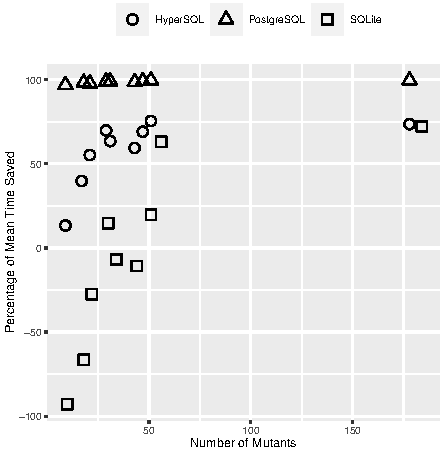
\includegraphics[scale=1.0]{graphics/graphic_scatterplot_nummutants_percentage.pdf}
  \caption{Box plot of the execution time for the original and virtual mutation analysis techniques.}
  \label{fig:graphic_bwplot_schema_analysistime_org_vm}

  % Details about the box plot from the R documentation:

  % The lower and upper "hinges" correspond to the first and third quartiles (the 25th and 75th percentiles). This differs
  % slightly from the method used by the boxplot function, and may be apparent with small samples. See boxplot.stats for for
  % more information on how hinge positions are calculated for boxplot.

  % The upper whisker extends from the hinge to the highest value that is within 1.5 * IQR of the hinge, where IQR is the
  % inter-quartile range, or distance between the first and third quartiles. The lower whisker extends from the hinge to
  % the lowest value within 1.5 * IQR of the hinge. Data beyond the end of the whiskers are outliers and plotted as points
  % (as specified by Tukey).

  % Commentary on the results in this output:

  % - Note that this data has been "log transformed" using a log-to-the-base-ten transformation
  % - Transformation is done because the Postgres-Original data is on a different scale than all other data
  % - This means that you will only see variation for Postgres-Original (without transformation)
  % - Using the log-transformed data shows the basic trends in the data sets

  {\small \justifying{ \noindent In this plot the box itself represents the interquartile range (IQR), or the measure of
      statistical dispersion that is the difference between the first and third quartiles. Furthermore, the upper
      whisker extends from the top of the box to the highest value that is within 1.5 times the IQR, the lower whisker
      goes from the bottom of the box to the lowest value within 1.5 times the IQR, and the thick horizontal line
      represents the median value. The boxes in this plot are noticeably compressed because there is little variance in
      the timings across the different configurations.  Since the results from running the original method on the
      \Postgres DBMS differ substantially from those with the other techniques and databases, all of the
      data values were log-transformed, thereby best revealing the relevant trends.} \par}

\end{figure*}








% PURPOSE: Compare the virtual and time-constrained techniques in terms of their mutation score and the number of
% mutants that are actually executed during mutation analysis, showing the superiority of virtual mutation.

\subsubsection{Virtual and Time-Constrained Mutation}
\label{sec:empirical-study-RQ-virtual-time-constrained-virtual}
% vim: ft=tex
%!TEX root=ast2016.tex

% GRAPHIC: This is the box and whisker plot that shows the mutation score for the two techniques
%!TEX root=ast2016.tex

\begin{figure*}[t]
  \centering
  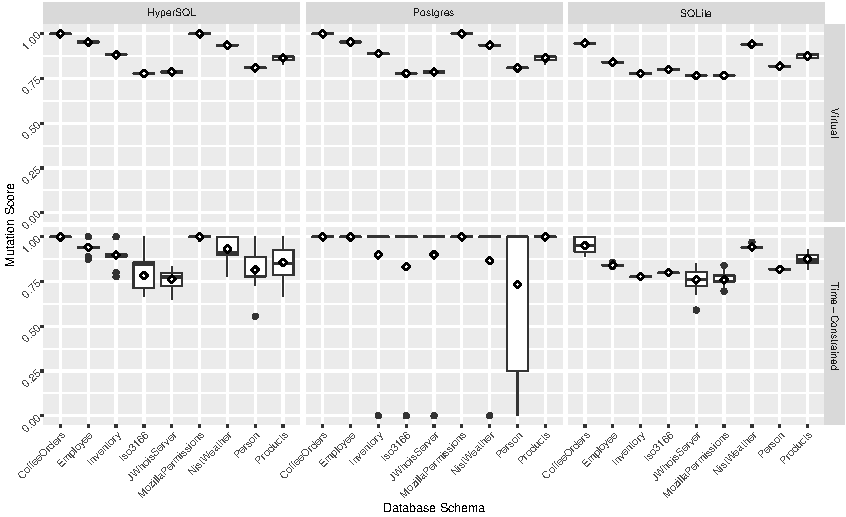
\includegraphics[scale=1.0]{graphics/graphic_bwplot_schema_mutationscore_vm_tcm.pdf}
  \caption{Box plot of the mutation score for the virtual and time-constrained mutation analysis techniques.}\label{fig:graphic_bwplot_schema_mutationscore_vm_tcm}

  % NOTE: This caption is not yet correct.

  {\small \justifying{\noindent The meaning for this box plot's elements is the same as the meaning of those described
      in the subcaption of Figure~\ref{fig:graphic_bwplot_schema_analysistime_org_vm}. Additionally, in this box plot a
      filled circle denotes an outlier and the open diamond is the mean value. Using test suites from thirty separate
      runs of the search-based test data generation method developed by McMinn \etal~\cite{McMinn2015}, this plot shows
      the variation in the mutation score for both the virtual and the time-constrained method and for all of the chosen
  relational schemas and the three database management systems. } \par}

\end{figure*}


% GRAPHIC: This is the bar chart of the number of mutants that each technique ran during mutation analysis
% NOTE: This graph was removed due to space constraints, it can be summarized in the text, I think.
% %!TEX root=ast2016.tex

\begin{figure*}[t]
  \centering
  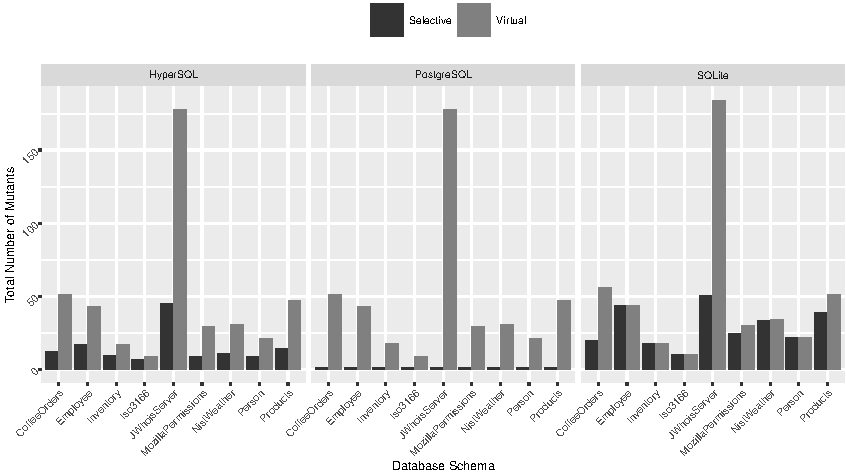
\includegraphics[scale=1.0]{graphics/graphic_barplot_schema_mutantcount_vm_tcm.pdf}
  \caption{Bar plot of the mutant count for both the virtual and time-constrained mutation analysis techniques.}
  \label{fig:graphic_barplot_schema_mutantcount_vm_tcm}

  {\small \justifying{ \noindent In this plot the height of the bar corresponds to the number of mutants subject to
      analysis by the virtual and time-constrained methods; this count is reported for all of the chosen relational
      schemas and the three database management systems. Since the time-constrained technique employs randomness to
      select mutants that can be run within a specified time limit, the height of a light grey bar is the average across
      a total of thirty runs; virtual mutation analysis is deterministic and thus the height of the dark grey bar is a
      direct count. } \par}

\end{figure*}


\inlineheading{Virtual and Time-Constrained Mutation} Since the experiments revealed that \vma~is faster than the \Original~one in $22$ out of the $27$ studied configurations --- and competitive with the DBMS-based method in the other $5$ --- it is useful to ascertain whether the presented technique might yield more accurate mutation scores in some circumstances. To this end, Figure~\ref{fig:graphic_bwplot_schema_mutationscore_vm_tcm} presents the mutation score of both the virtual approach and a time-limited analysis in which \Original~randomly analyses mutants for as long as virtual. These box plots show that the time-constrained technique results in mutation scores that are often highly variable. This result can be attributed to randomness inherent in running mutation analysis under a strict time limit that will not permit the examination of every mutant. For instance, the noticeable variability in mutation score when the Person schema is run on \Postgres~is due to the possibility of not finishing the analysis of the first mutant.

Bearing in mind that the virtual method produces mutation scores that are always equal to those achieved by the standard technique, it is also important to observe that time-constrained mutation analysis leads to overly high mutation scores.  Yet, at least for the \HyperSQL~and \SQLite~DBMSs, the box plots in Figure~\ref{fig:graphic_bwplot_schema_mutationscore_vm_tcm} suggest that the mutation scores are roughly similar for \vma~and the time-constrained method. To rigorously establish this correlation, we calculated Kendall's \taub~for the two techniques on each of the DBMSs, arriving at the values of $0.561$ (moderate), $0.132$ (low) and $0.756$ (high) for \HyperSQL, \PostgreSQL and \sqlite, respectively. These correlations suggest that virtual mutation is the best option when highly accurate scores are needed and there is limited time for mutation analysis of a database schema.

% These correlations suggest that the time-constrained mutation
% analysis of a schema for fast, in-memory databases like \HyperSQL~and \sqlite~leads to scores that respectively have a
% moderate and high correlation with the actual score. Yet, the scores produced by virtual and time-constrained mutation
% analysis on \postgres~have a low correlation. Overall, these results indicate that virtual mutation is the best option




